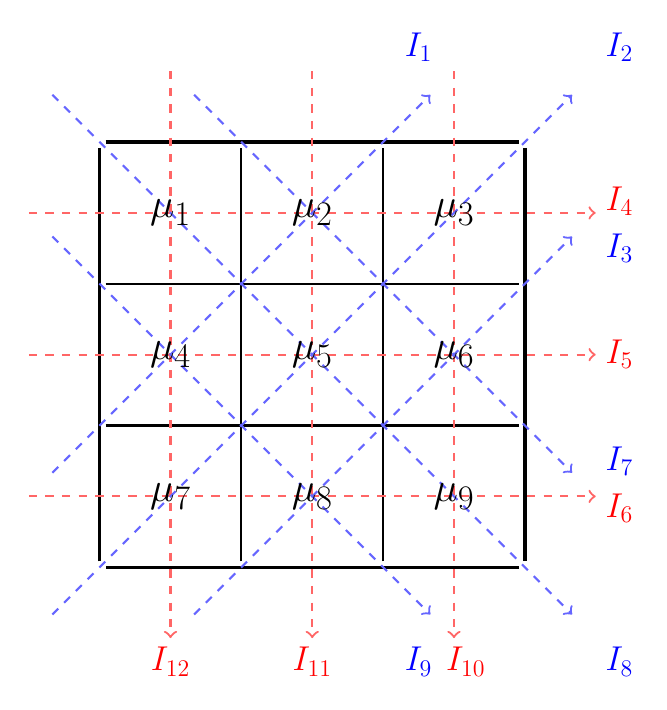
\begin{tikzpicture}[scale=0.6, every node/.style={scale=0.6}]
    % Kästchen
    \node (A1) at (0,0) {};
    \node (B1) at (0,3) {};
    \node (C1) at (0,6) {};
    \node (D1) at (0,9) {};
    \node (A2) at (3,0) {};
    \node (B2) at (3,3) {};
    \node (C2) at (3,6) {};
    \node (D2) at (3,9) {};
    \node (A3) at (6,0) {};
    \node (B3) at (6,3) {};
    \node (C3) at (6,6) {};
    \node (D3) at (6,9) {};
    \node (A4) at (9,0) {};
    \node (B4) at (9,3) {};
    \node (C4) at (9,6) {};
    \node (D4) at (9,9) {};

    \node (E1) at (0,0) {};
    \node (E2) at (0,9) {};
    \node (E3) at (9,9) {};
    \node (E4) at (9,0) {};


    % Umrandung
    \draw[very thick] (E1) to (E2) to (E3) to (E4) to (E1);
    \draw[thick] (B1) to (B4);
    \draw[thick] (C1) to (C4);
    \draw[thick] (A2) to (D2);
    \draw[thick] (A3) to (D3);

    % gerade Projektionen
    \draw[->, red!60, thick, dashed] (-1.5, 7.5) to (10.5, 7.5);
    \draw[->, red!60, thick, dashed] (-1.5, 4.5) to (10.5, 4.5);
    \draw[->, red!60, thick, dashed] (-1.5, 1.5) to (10.5, 1.5);

    \draw[->, red!60, thick, dashed] (1.5, 10.5) to (1.5, -1.5);
    \draw[->, red!60, thick, dashed] (4.5, 10.5) to (4.5, -1.5);
    \draw[->, red!60, thick, dashed] (7.5, 10.5) to (7.5, -1.5);

    % quere Projektionen
    \draw[->, blue!60, thick, dashed] (-1, -1) to (10, 10);
    \draw[->, blue!60, thick, dashed] (-1, 2) to (7, 10);
    \draw[->, blue!60, thick, dashed] (2, -1) to (10, 7);

    \draw[->, blue!60, thick, dashed] (2, 10) to (10, 2);
    \draw[->, blue!60, thick, dashed] (-1, 10) to (10, -1);
    \draw[->, blue!60, thick, dashed] (-1, 7) to (7, -1);

    % Erklärungsnodes
    \node [blue] at (6.75, 11) {\huge$I_{1}$};
    \node [blue] at (11, 11) {\huge$I_{2}$};
    \node [red] at (11, 7.75) {\huge$I_{4}$};
    \node [blue] at (11, 6.75) {\huge$I_{3}$};
    \node [red] at (11, 4.5) {\huge$I_{5}$};
    \node [blue] at (11, 2.25) {\huge$I_{7}$};
    \node [red] at (11, 1.25) {\huge$I_{6}$};
    \node [blue] at (11, -2) {\huge$I_{8}$};
    \node [red] at (7.75, -2) {\huge$I_{10}$};
    \node [blue] at (6.75, -2) {\huge$I_{9}$};
    \node [red] at (1.5, -2) {\huge$I_{12}$};
    \node [red] at (4.5, -2) {\huge$I_{11}$};

    %mu's
    \node at (1.5, 7.5) {\Huge$\mu_{1}$};
    \node at (4.5, 7.5) {\Huge$\mu_{2}$};
    \node at (7.5, 7.5) {\Huge$\mu_{3}$};

    \node at (1.5, 4.5) {\Huge$\mu_{4}$};
    \node at (4.5, 4.5) {\Huge$\mu_{5}$};
    \node at (7.5, 4.5) {\Huge$\mu_{6}$};

    \node at (1.5, 1.5) {\Huge$\mu_{7}$};
    \node at (4.5, 1.5) {\Huge$\mu_{8}$};
    \node at (7.5, 1.5) {\Huge$\mu_{9}$};
  \end{tikzpicture}
